\documentclass[conference]{IEEEtran}
\usepackage[T1]{fontenc}
\usepackage[utf8]{inputenc}
\usepackage[spanish,es-tabla]{babel}
\usepackage{amsmath,amssymb}
\usepackage{graphicx}
\usepackage{booktabs}
\usepackage{xcolor}
\usepackage{listings}
\usepackage[hidelinks]{hyperref}
\usepackage[left=2cm,right=2cm,top=2cm,bottom=2cm]{geometry}

\lstset{language=VHDL,basicstyle=\ttfamily\footnotesize,
  frame=single,breaklines=true,columns=fullflexible,
  keepspaces=true,showstringspaces=false,captionpos=b}

\begin{document}

\title{Electrónica Digital 2: Laboratorio 2\\
ALU: lógica combinacional y diseño jerárquico}
\author{
\IEEEauthorblockN{Isaac Martirena}
\IEEEauthorblockA{Equipo UTEC City\\
\textit{Ingeniería en Mecatrónica}\\
\textit{Universidad Tecnológica (UTEC)}\\
Fray Bentos, Uruguay\\
isaac.martirena@estudiantes.utec.edu.uy}
\and
\IEEEauthorblockN{Hector Pereira}
\IEEEauthorblockA{Equipo UTEC City\\
\textit{Ingeniería en Mecatrónica}\\
\textit{Universidad Tecnológica (UTEC)}\\
Fray Bentos, Uruguay\\
hector.pereira@estudiantes.utec.edu.uy}}

\maketitle

\begin{abstract}
\end{abstract}

\begin{IEEEkeywords}
VHDL, ALU, lógica combinacional, diseño jerárquico, testbench.
\end{IEEEkeywords}


\section{Introducción}

Una unidad aritmético-lógica (ALU) reúne operaciones aritméticas,
lógicas y de comparación en un circuito cuya salida se selecciona
mediante un código de operación. Su descripción en VHDL permite
estudiar tanto el comportamiento combinacional como la organización
interna del hardware y su verificación mediante simulación.

El Laboratorio 2 de Electrónica Digital 2 propone una ALU de
dieciséis operaciones, con dos operandos sin signo de cuatro bits,
un resultado del mismo ancho y las banderas Carry y Zero. El trabajo
se divide en una descripción monolítica, Parte A, y una
reestructuración jerárquica, Parte B, que conserva la interfaz y el
comportamiento de la primera versión~\cite{guialab2}.

Esta organización permite relacionar la especificación funcional
con dos formas de describir el mismo sistema. Además de comprobar
las operaciones, interesa analizar cómo la división en módulos
facilita reutilizar un sumador y verificar cada bloque antes de
integrarlo en la ALU completa.

\subsection{Objetivos}
\begin{itemize}
\item Describir una ALU combinacional de dieciséis operaciones
utilizando el paquete \texttt{numeric\_std}.
\item Implementar las banderas de estado y verificar los casos de
borde de la aritmética de cuatro bits.
\item Reorganizar el diseño mediante componentes, reutilizando un
único sumador dentro de la unidad aritmética.
\item Verificar cada módulo y el sistema completo mediante bancos
de prueba autoverificables.
\item Contrastar las dos versiones y validar su funcionamiento en
la placa Spartan Edge Accelerator con el shield UTEC.
\end{itemize}


\section{Marco teórico}

\subsection{Lógica combinacional y descripción en VHDL}
En un circuito combinacional, las salidas dependen de las entradas
actuales y no de un estado almacenado. En VHDL, la entidad define
los puertos y la arquitectura describe el comportamiento o las
conexiones entre los bloques. Aunque las instrucciones dentro de un
proceso se evalúan en orden, los procesos y las asignaciones
concurrentes representan circuitos que operan en paralelo~\cite{fundamentos}.

Un proceso combinacional debe ser sensible a todas las señales que
lee y asignar sus salidas para cada alternativa de ejecución. Las
asignaciones incompletas pueden inferir latches, mientras que una
lista de sensibilidad incompleta puede producir diferencias entre
la simulación y el hardware sintetizado. Una sentencia \texttt{case}
con valores por defecto y una rama \texttt{when others} permite
describir de forma completa la selección por opcode~\cite{combinacional}.

Las variables, asignadas con \texttt{:=}, actualizan su valor
inmediatamente dentro del proceso. Las señales, asignadas con
\texttt{<=}, programan una actualización posterior. Esta diferencia
resulta relevante al calcular un resultado temporal y derivar de
él una bandera dentro del mismo proceso~\cite{fundamentos}.

\subsection{Tipos numéricos y aritmética de cuatro bits}
El paquete \texttt{ieee.std\_logic\_1164} define los tipos
\texttt{std\_logic} y \texttt{std\_logic\_vector}. El paquete
\texttt{ieee.numeric\_std} incorpora los tipos \texttt{unsigned} y
\texttt{signed}, que hacen explícita la interpretación numérica de
los vectores y permiten aplicar operaciones aritméticas y
comparaciones~\cite{combinacional}. En este laboratorio se utiliza
la interpretación sin signo indicada en la consigna.

Un operando sin signo de cuatro bits representa valores entre
$0$ y $2^4-1=15$. Si se conservan únicamente los cuatro bits menos
significativos de un resultado aritmético, el valor se reduce
módulo $16$. Por ejemplo, $15+1$ produce \texttt{0000} con acarreo,
y $0-1$ produce \texttt{1111} con préstamo. El resultado binario
de la resta sigue siendo un vector sin signo; no representa un
número negativo bajo esta interpretación~\cite{casoalu}.

Para obtener el acarreo de una suma es necesario extender los
operandos antes de operar. Si $T$ es el resultado extendido:
\begin{equation}
T=(0\mathbin{\&}A)+(0\mathbin{\&}B),\qquad
R=T(3\!:\!0),\quad C=T(4),
\end{equation}
donde $\&$ indica concatenación. La extensión conserva el quinto
bit que se perdería al calcular directamente en cuatro bits.

\subsection{Banderas de estado}
Según la especificación, Carry expresa el acarreo de salida en
$A+B$ y el préstamo (\textit{borrow}) en $A-B$. En la resta sin
signo existe préstamo cuando $A<B$. Para las operaciones lógicas
y las comparaciones, la consigna fija Carry en cero~\cite{guialab2}.
El acarreo sin signo y el desbordamiento de una operación con signo
son condiciones diferentes y dependen de la interpretación de los bits.
Para las operaciones restantes se adopta la convención de la
Tabla~\ref{tab:carry}: acarreo al incrementar, préstamo al decrementar
o calcular $0-X$, y bit descartado en los desplazamientos lógicos.
Esta extensión es una decisión de diseño del equipo.

Zero se obtiene del resultado final:
\begin{equation}
Z=\begin{cases}
1,& R=\texttt{0000},\\
0,& R\ne\texttt{0000}.
\end{cases}
\end{equation}
Por tanto, Zero no indica por sí sola si los operandos son iguales.
En la operación de comparación $A=B$, un resultado verdadero se
codifica como \texttt{0001} y deja Zero en cero.

\subsection{Complemento a dos y reutilización del sumador}
Para un vector $X$ de cuatro bits, su complemento a dos corresponde
a $(-X)\bmod16$ y se obtiene invirtiendo sus bits y sumando uno.
La misma identidad permite expresar una resta como una suma:
\begin{equation}
A-B\equiv A+\overline{B}+1\pmod{16}.
\end{equation}
Un sumador con entrada de acarreo permite implementar suma, resta,
incremento, decremento y complemento a dos mediante la selección de
sus operandos y de \texttt{cin}. La consigna utiliza esta propiedad
para reutilizar una sola instancia de \texttt{adder4} en la unidad
aritmética~\cite{guialab2}. En la resta implementada mediante
$A+\overline{B}+1$, el acarreo de salida indica ausencia de préstamo;
la bandera borrow corresponde a su negación.

\subsection{Diseño jerárquico}
El diseño jerárquico divide un sistema en bloques con interfaces
definidas. Las declaraciones \texttt{component} describen los
puertos de los componentes y las instancias con \texttt{port map}
los conectan mediante señales internas~\cite{jerarquia}.
En una ALU, distintos bloques pueden producir resultados en paralelo
y un multiplexor selecciona la salida correspondiente al
opcode~\cite{casoalu}.

La metodología top-down parte de la función global para definir
bloques e interfaces. La implementación bottom-up comienza por los
bloques básicos y avanza hacia su integración. Esta combinación
permite comprobar cada módulo y localizar errores antes de verificar
el sistema completo. La división en archivos o componentes no
garantiza por sí sola una reducción de recursos o retardos; esos
aspectos requieren evaluar el diseño sintetizado.

\subsection{Testbench y verificación}
Un banco de pruebas instancia el circuito bajo prueba, genera
estímulos y comprueba sus salidas. Las sentencias \texttt{assert}
permiten detectar diferencias respecto de un resultado esperado,
acompañadas de un mensaje que identifique el caso~\cite{fundamentos,casoalu}.
El banco no forma parte del hardware implementado.

La ALU tiene $16\times16\times16=4096$ combinaciones binarias de
opcode, $A$ y $B$. Este espacio permite plantear una comprobación
exhaustiva del resultado y de las banderas. El sumador de cuatro
bits con \texttt{cin} presenta $16\times16\times2=512$
combinaciones. Comparar ambas ALU comprueba su equivalencia, pero
tambi\'en se necesita un modelo de referencia independiente para
detectar errores compartidos por las dos versiones.


\section{Metodología}

\subsection{Materiales y herramientas previstos}
La consigna establece el uso de una Spartan Edge Accelerator Board
con FPGA Spartan-7 XC7S15, el shield multifunción UTEC, cable USB-C
y programador JTAG HS2. El entorno de referencia es Vivado 2025.1;
EDA Playground se admite como alternativa para la simulación
funcional~\cite{guialab2}. La versión y el equipamiento efectivamente
utilizados se registrarán al desarrollar las pruebas.

\subsection{Especificación de la interfaz}
Ambas partes conservan la entidad \texttt{alu}. El bus de doce bits
\texttt{SW} contiene los operandos y el opcode, según la
Tabla~\ref{tab:interfaz}. Las salidas son \texttt{Result}, de cuatro
bits, y las banderas \texttt{Carry} y \texttt{Zero}, de un bit cada
una. La señal \texttt{AR\_3V3\_EN} debe mantenerse en
\texttt{'0'} y asignarse al pin L13 para habilitar los 3,3 V de los
dip-switches; el estándar de E/S indicado es
\texttt{LVCMOS33}~\cite{guialab2}.

La Figura~\ref{fig:alu_parte_a} presenta la vista general de la
Parte A: separación del bus de entrada, bloque combinacional de
la ALU y conexiones con los LEDs y la habilitación del shield.

\begin{figure*}[!t]
\centering
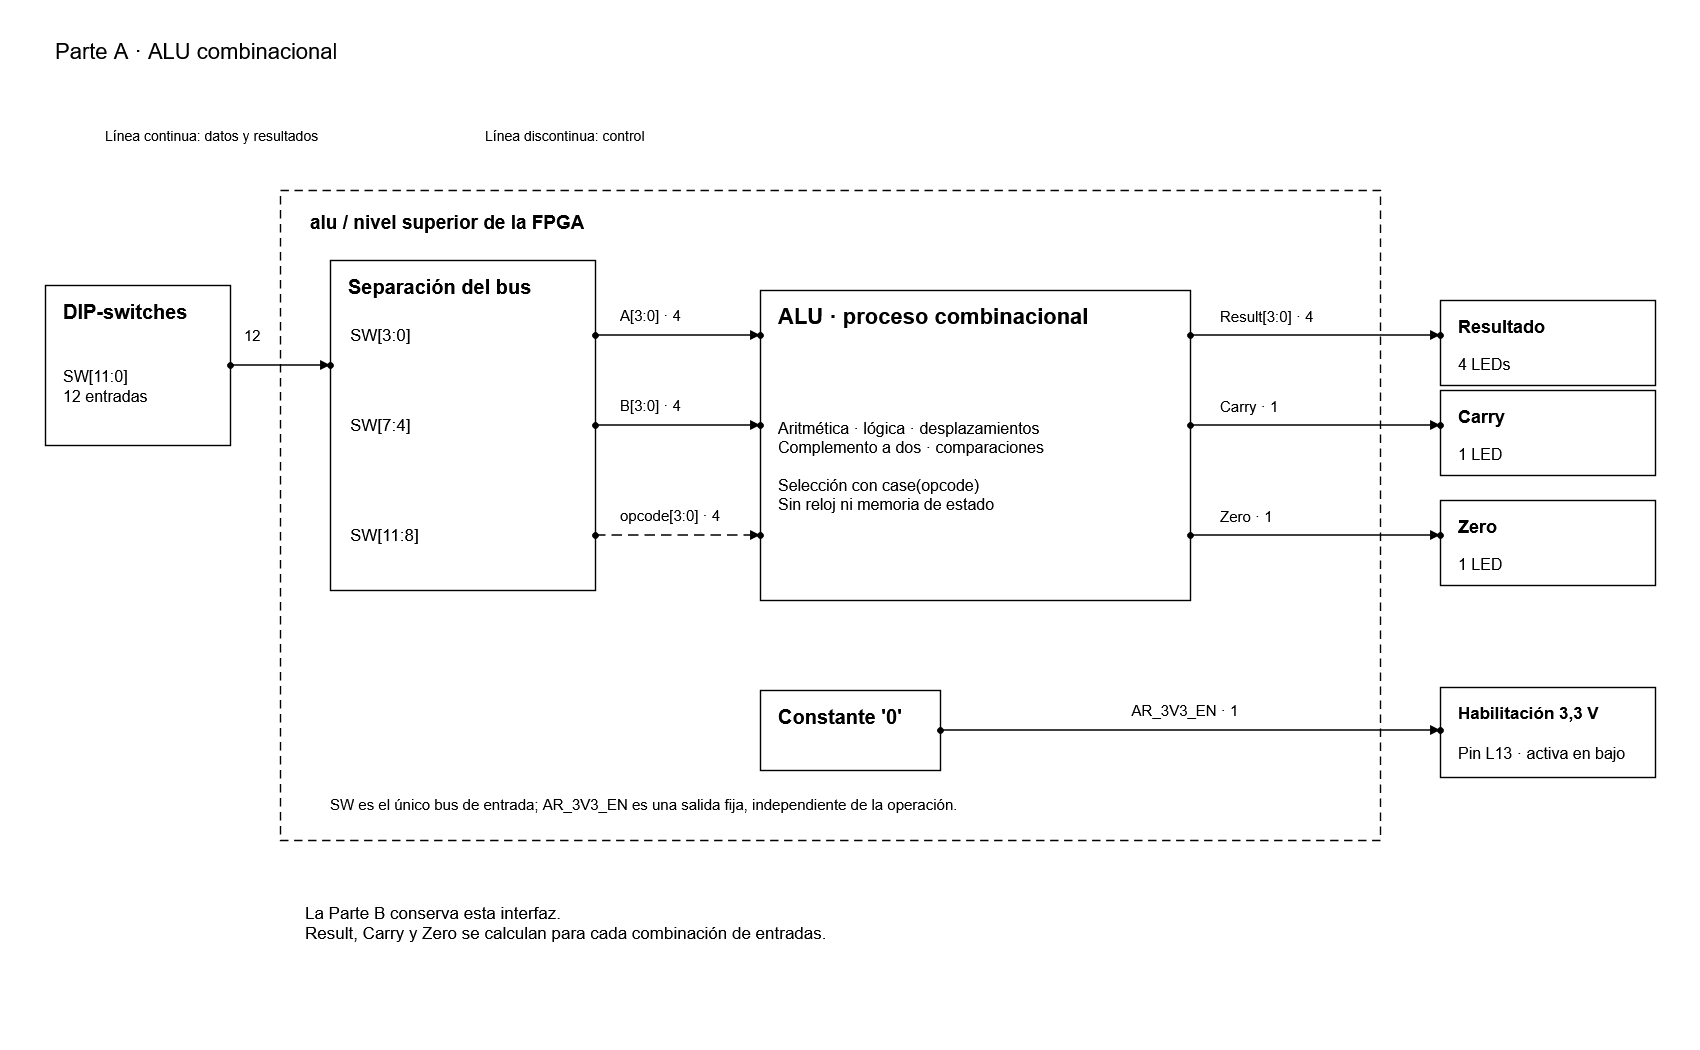
\includegraphics[width=\textwidth]{imagenes/alu_parte_a.png}
\caption{Vista general de la ALU monolítica y su interfaz con el shield UTEC (Parte A).}
\label{fig:alu_parte_a}
\end{figure*}

\begin{table}[htbp]
\centering
\caption{Organización del bus de entrada}
\label{tab:interfaz}
\begin{tabular}{lll}
\toprule
Campo & Bits de \texttt{SW} & Ancho\\
\midrule
$A$ & \texttt{3 downto 0} & 4 bits\\
$B$ & \texttt{7 downto 4} & 4 bits\\
Opcode & \texttt{11 downto 8} & 4 bits\\
\bottomrule
\end{tabular}
\end{table}

\subsection{Operaciones requeridas}
La Tabla~\ref{tab:operaciones} reproduce las operaciones definidas
en la consigna~\cite{guialab2}. Los desplazamientos son lógicos,
de una posición, y las comparaciones devuelven \texttt{0001}
cuando la condición se cumple y \texttt{0000} en caso contrario.

\begin{table}[htbp]
\centering
\caption{Operaciones de la ALU}
\label{tab:operaciones}
\small
\begin{tabular}{cll}
\toprule
Opcode & Operación & Función\\
\midrule
\texttt{0000} & $A+B$ & Suma\\
\texttt{0001} & $A-B$ & Resta\\
\texttt{0010} & $A\mathbin{\mathrm{AND}}B$ & AND bit a bit\\
\texttt{0011} & $A\mathbin{\mathrm{OR}}B$ & OR bit a bit\\
\texttt{0100} & $A\mathbin{\mathrm{XOR}}B$ & XOR bit a bit\\
\texttt{0101} & $\mathrm{NOT}\ A$ & Inversión de bits\\
\texttt{0110} & $A\ll1$ & Desplazamiento izquierdo\\
\texttt{0111} & $A\gg1$ & Desplazamiento derecho\\
\texttt{1000} & $A+1$ & Incremento de $A$\\
\texttt{1001} & $A-1$ & Decremento de $A$\\
\texttt{1010} & $B+1$ & Incremento de $B$\\
\texttt{1011} & $B-1$ & Decremento de $B$\\
\texttt{1100} & $\mathrm{comp2}(A)$ & Complemento a dos de $A$\\
\texttt{1101} & $\mathrm{comp2}(B)$ & Complemento a dos de $B$\\
\texttt{1110} & $A=B$ & Comparación de igualdad\\
\texttt{1111} & $A>B$ & Comparación de magnitud\\
\bottomrule
\end{tabular}
\end{table}

\subsection{Organización del desarrollo}
En la Parte A se describió la ALU en \texttt{alu.vhd}, mediante un
único proceso combinacional sensible a $A$, $B$ y opcode, con
selección mediante \texttt{case}. Se asignaron valores por defecto
a las variables temporales y se calculó Zero a partir del resultado
de la operación. La segunda etapa prevé reorganizar el sistema en \texttt{adder4},
\texttt{arith\_unit}, \texttt{logic\_unit}, \texttt{shift\_unit}
y \texttt{compare\_unit}, conectados desde un nivel superior
estructural. La unidad aritmética utilizará una sola instancia
del sumador. Se prevé verificar los bloques por separado y después
reutilizar los estímulos de la Parte A para contrastar la ALU completa.

La Figura~\ref{fig:alu_parte_b} muestra la arquitectura propuesta
para la Parte B. Los módulos aritmético, lógico, de desplazamiento
y de comparación producen resultados intermedios; la selección
controlada por opcode determina el resultado final y Carry.
Zero se calcula a partir del resultado seleccionado.

Para verificar la Parte A se implementó \texttt{tb\_alu.vhd}, que
recorre los dieciséis opcodes y los dieciséis valores posibles de
cada operando. Cada estímulo se mantiene durante 10 ns antes de
comparar las salidas con un modelo de referencia basado en enteros.
Las comprobaciones con \texttt{assert} abarcan Result, Carry, Zero
y la salida fija de habilitación del shield. Este intervalo organiza
la simulación funcional; no representa una medición de retardo del
circuito físico.

\begin{figure*}[!t]
\centering
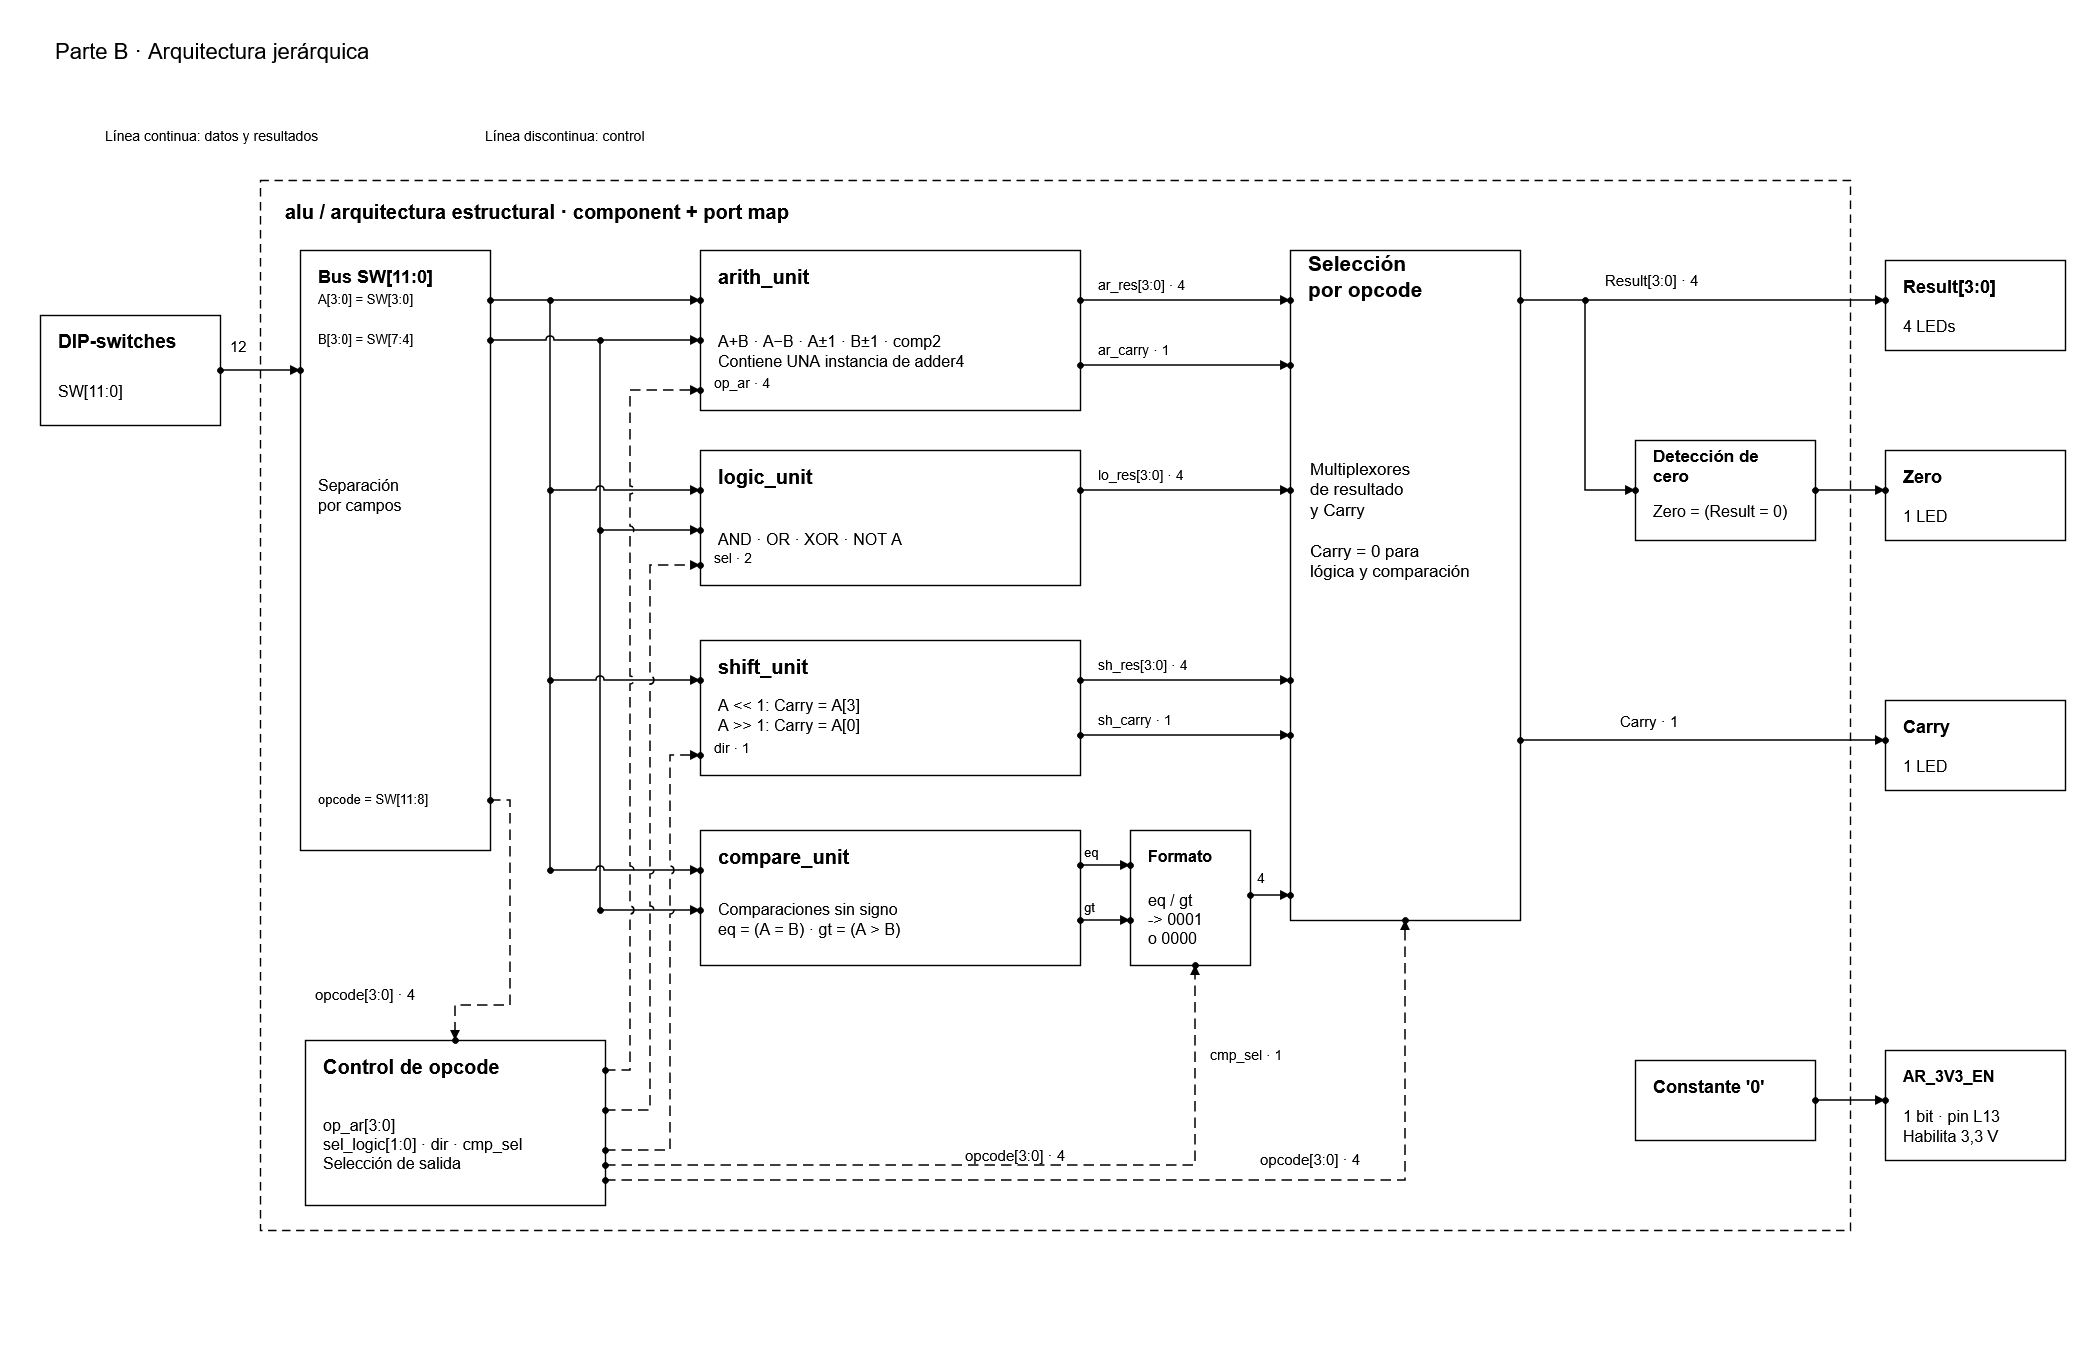
\includegraphics[width=\textwidth]{imagenes/alu_parte_b.png}
\caption{Arquitectura jerárquica de la Parte B: módulos, buses de datos, señales de control y selección de las salidas.}
\label{fig:alu_parte_b}
\end{figure*}

\subsection{Selección de operandos del sumador}
La Tabla~\ref{tab:operandos} define cómo obtener las ocho operaciones
aritméticas con un único sumador de cuatro bits. Las señales $x$ e
$y$ son los operandos seleccionados que se conectan a sus entradas
$a$ y $b$; \texttt{cin} aporta el acarreo de entrada. Los vectores
constantes y los operandos tienen cuatro bits, y la inversión se
realiza bit a bit. En todos los casos, el resultado corresponde a
los cuatro bits de salida $s$, mientras que \texttt{cout} se adapta
según la convención de banderas de la sección siguiente.

La Figura~\ref{fig:unidad_aritmetica} detalla la unidad aritmética:
la selección de operandos y la adaptación de la bandera rodean a
una única instancia de \texttt{adder4}. La tabla de selección
expresa las conexiones requeridas para cada operación, sin agregar
sumadores independientes.

\begin{figure*}[!t]
\centering
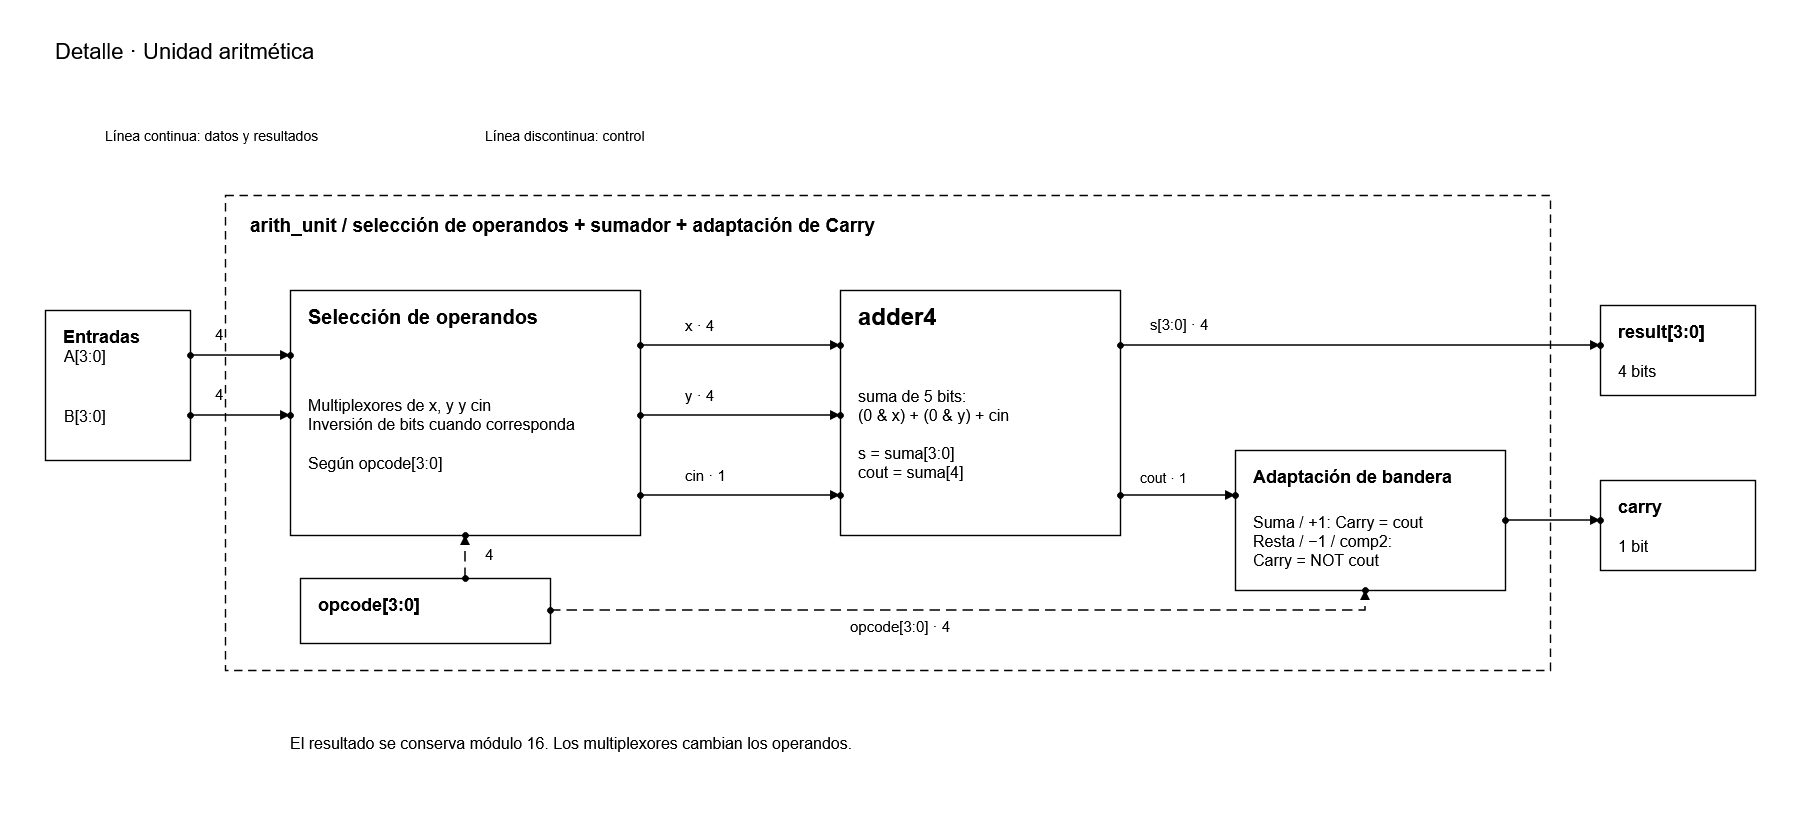
\includegraphics[width=\textwidth]{imagenes/unidad_aritmetica.png}
\caption{Detalle de la unidad aritmética de la Parte B: selección de operandos, sumador reutilizado y adaptación de Carry.}
\label{fig:unidad_aritmetica}
\end{figure*}

\begin{table}[htbp]
\centering
\caption{Selección de entradas del sumador reutilizado}
\label{tab:operandos}
\small
\setlength{\tabcolsep}{4pt}
\begin{tabular}{clcccc}
\toprule
Opcode & Operación & $x$ & $y$ & \texttt{cin} & Resultado\\
\midrule
\texttt{0000} & $A+B$ & $A$ & $B$ & 0 & $s(3:0)$\\
\texttt{0001} & $A-B$ & $A$ & $\overline{B}$ & 1 & $s(3:0)$\\
\texttt{1000} & $A+1$ & $A$ & \texttt{0000} & 1 & $s(3:0)$\\
\texttt{1001} & $A-1$ & $A$ & \texttt{1111} & 0 & $s(3:0)$\\
\texttt{1010} & $B+1$ & $B$ & \texttt{0000} & 1 & $s(3:0)$\\
\texttt{1011} & $B-1$ & $B$ & \texttt{1111} & 0 & $s(3:0)$\\
\texttt{1100} & $\mathrm{comp2}(A)$ & $\overline{A}$ & \texttt{0000} & 1 & $s(3:0)$\\
\texttt{1101} & $\mathrm{comp2}(B)$ & $\overline{B}$ & \texttt{0000} & 1 & $s(3:0)$\\
\bottomrule
\end{tabular}
\end{table}

\subsection{Convención adoptada para las banderas}
La consigna fija Carry para suma, resta, lógica y comparación,
pero no explicita su significado en las demás operaciones.
Para completar la especificación se adopta la
Tabla~\ref{tab:carry}. Se conserva el criterio de acarreo en
operaciones aditivas y de préstamo en las sustractivas. En la tabla,
$X$ representa el operando $A$ o $B$, según el opcode.

\begin{table}[htbp]
\centering
\caption{Convención adoptada para Carry}
\label{tab:carry}
\small
\begin{tabular}{ll}
\toprule
Operación & Carry vale 1 cuando\\
\midrule
$A+B$ & $A+B\geq16$\\
$A-B$ & $A<B$\\
$X+1$ & $X=15$\\
$X-1$ & $X=0$\\
$\mathrm{comp2}(X)$ & $X\ne0$ (préstamo de $0-X$)\\
Desplazamiento izquierdo & $A(3)=1$ (bit descartado)\\
Desplazamiento derecho & $A(0)=1$ (bit descartado)\\
Lógica y comparación & Nunca; Carry se mantiene en 0\\
\bottomrule
\end{tabular}
\end{table}

El complemento a dos se interpreta como $0-X$, conservando los
cuatro bits del resultado. Por ello, si $X\ne0$ se señala préstamo,
aunque el resultado mostrado sea un vector sin signo. Por ejemplo,
$\mathrm{comp2}(1)=\texttt{1111}$ con Carry en 1, mientras que
$\mathrm{comp2}(0)=\texttt{0000}$ con Carry en 0.

Con la selección de operandos del sumador reutilizado, la adaptación
es Carry igual a \texttt{cout} para suma e incrementos, y Carry
igual a \texttt{not cout} para resta, decrementos y complemento a dos.
Esta regla distingue el acarreo bruto del sumador de la bandera
que se expone en la interfaz.

Los desplazamientos introducen un cero en la posición vacante y
copian a Carry el bit que abandona el vector. Así, desplazar
\texttt{1000} una posición a la izquierda produce \texttt{0000}
con Carry en 1; desplazar \texttt{0001} a la derecha da la misma
combinación de resultado y Carry. Zero vale 1 en ambos ejemplos
porque siempre se calcula sobre los cuatro bits del resultado final,
independientemente de Carry.

Esta convención se aplicará a las Partes A y B y al modelo de
referencia de sus bancos de prueba.


\section{Resultados y discusión}

\subsection{Verificación funcional de la Parte A}
El testbench autoverificable se ejecutó en XSim 2025.1 y completó
las 4096 combinaciones binarias de entrada: 256 por cada opcode.
No se detectaron diferencias en Result, Carry, Zero ni en la salida
\texttt{AR\_3V3\_EN}. El último caso se comprobó a los
$40{,}96\,\mu\mathrm{s}$, de acuerdo con los 10 ns asignados a cada
estímulo. El registro terminó con el mensaje
\texttt{PASS: 4096 casos verificados}.

La Figura~\ref{fig:ondas_a_general} muestra el recorrido completo
de la simulación. A esa escala, los cambios de los buses se ven
superpuestos; para interpretar los valores se ampliaron dos casos
de borde en la Figura~\ref{fig:ondas_a_bordes}. Los valores de los
buses se presentan en hexadecimal, con \texttt{SW} organizado como
opcode, $B$ y $A$, de mayor a menor peso.

En el primer caso, a los 2410 ns, \texttt{SW=01f} selecciona
$A=15$, $B=1$ y la suma. Se obtiene \texttt{Result=0},
\texttt{Carry=1} y \texttt{Zero=1}: el resultado matemático es 16,
pero se conservan cuatro bits y el acarreo indica el desbordamiento
sin signo. En el segundo, a los 2570 ns, \texttt{SW=110} selecciona
$A=0$, $B=1$ y la resta. El resultado es \texttt{f} (15),
con \texttt{Carry=1} por préstamo y \texttt{Zero=0}.
En ambos casos la habilitación \texttt{AR\_3V3\_EN} permanece en cero.

\begin{figure*}[!t]
\centering
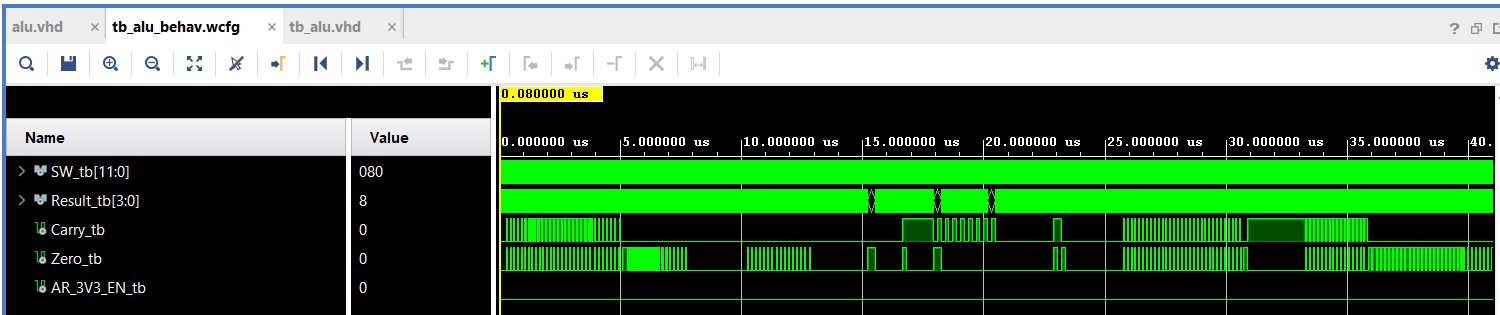
\includegraphics[width=\textwidth]{imagenes/ondas_parte_a_completa.png}
\caption{Simulación funcional completa de la Parte A: 4096 combinaciones de entrada en 40,96 microsegundos.}
\label{fig:ondas_a_general}
\end{figure*}

\begin{figure*}[!t]
\centering
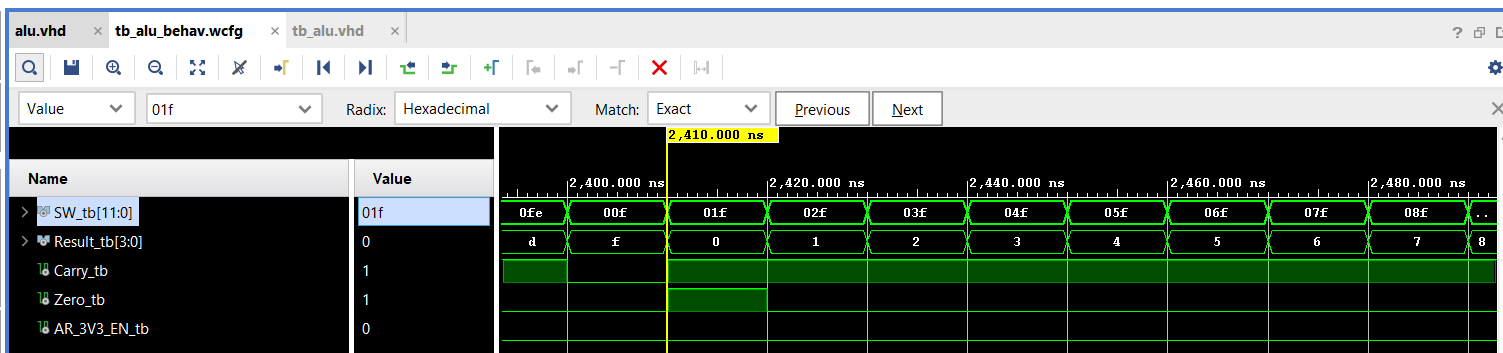
\includegraphics[width=\textwidth]{imagenes/ondas_parte_a_suma_acarreo.png}
\par\medskip
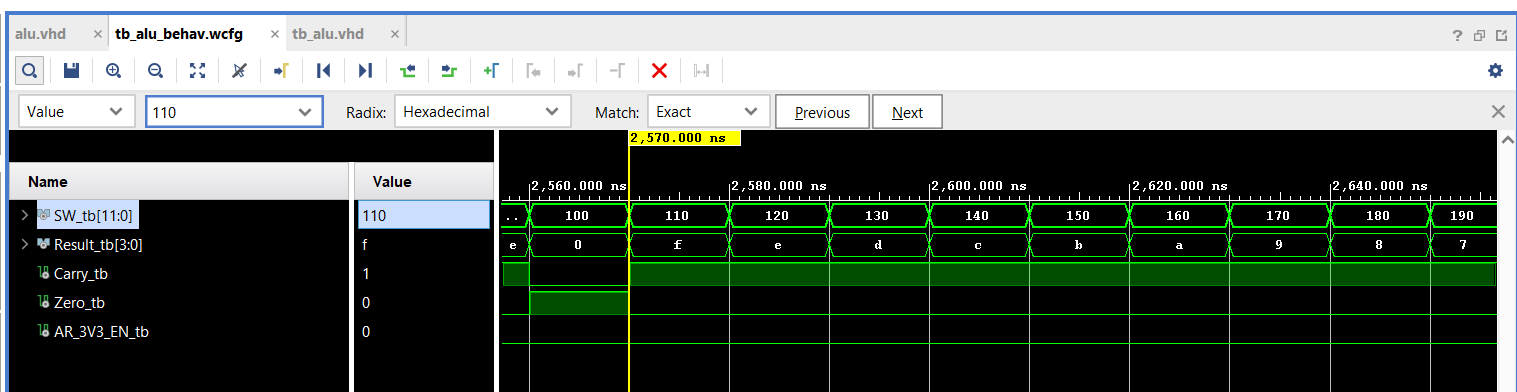
\includegraphics[width=\textwidth]{imagenes/ondas_parte_a_resta_prestamo.png}
\caption{Casos de borde de la Parte A. Arriba: $15+1$, con acarreo y resultado cero. Abajo: $0-1$, con préstamo y resultado de cuatro bits igual a 15.}
\label{fig:ondas_a_bordes}
\end{figure*}

\subsection{Síntesis preliminar de la Parte A}
La síntesis para \texttt{xc7s15ftgb196-1} terminó sin errores ni
advertencias críticas. El reporte de utilización informa 33 Slice
LUTs, seis multiplexores F7 y uno F8; los registros, latches, bloques
de RAM y DSP utilizados son cero. La ausencia de almacenamiento es
coherente con la descripción combinacional prevista. La advertencia
sobre \texttt{AR\_3V3\_EN} conectada a cero corresponde a la
habilitación fija requerida por el shield.

Estos resultados corresponden a simulación funcional y síntesis
sin restricciones XDC. La asignación de pines, la implementación,
la verificación temporal y las pruebas en placa de la Parte A
todavía no se realizaron.


\section{Preguntas del laboratorio}


\section{Conclusiones}


\begin{thebibliography}{00}
\bibitem{guialab2} UTEC, ``Laboratorio 2. ALU: lógica combinacional
y diseño jerárquico. Partes A y B,'' Electrónica Digital 2,
Ingeniería Mecatrónica, guía de laboratorio, 2026.

\bibitem{combinacional} UTEC, ``Lógica combinacional en FPGA,''
Electrónica Digital 2, material de clase disponible en Moodle,
2026, pp. 3--5 y 27--28.

\bibitem{fundamentos} UTEC, ``VHDL: fundamentos del lenguaje,''
Electrónica Digital 2, material de clase disponible en Moodle,
2026, pp. 22--28, 34--37 y 42--47.

\bibitem{jerarquia} UTEC, ``Diseño jerárquico,'' Electrónica
Digital 2, material de clase disponible en Moodle, 2026,
pp. 4--18.

\bibitem{casoalu} UTEC, ``Una ALU como caso de estudio completo,''
Electrónica Digital 2, material de clase disponible en Moodle,
2026, pp. 3--5 y 29--41.
\end{thebibliography}


\end{document}
